%##########################  CHAPER 6: APPLICATION  #######################

\chapter{Entwicklung der Anwendung}\label{kap:application}

Dieses Kapitel beschreibt die Entwicklung der Anwendung, als 
autonomes System welches auf dem Raspberry Pi läuft, 
Bilder über eine infrarotfähige Kamera aufnimmt und diese
auf dem Neural Compute Stick 2 mit dem trainierten Modell 
inferiert.
Desweiteren wird die Implementierung der verbindugn zu einem 
Host Pc beschrieben.


%-------------------------  SECTION 1: AUFBAU  ------------------------
\section{Aufbau/Hardware}\label{sec:aufbau}

Im folgenden werden die zur Realisierung der Anwendung verwendeten 
Komponenten erläutert.

\subsection*{Raspberry Pi}
Der Anwendungs Code läuft auf dem Raspberry Pi. 
Der Neural Compute Stick 2 wird über eine USB Schnittstelle verbunden.


\begin{figure}[H]
    \centering
    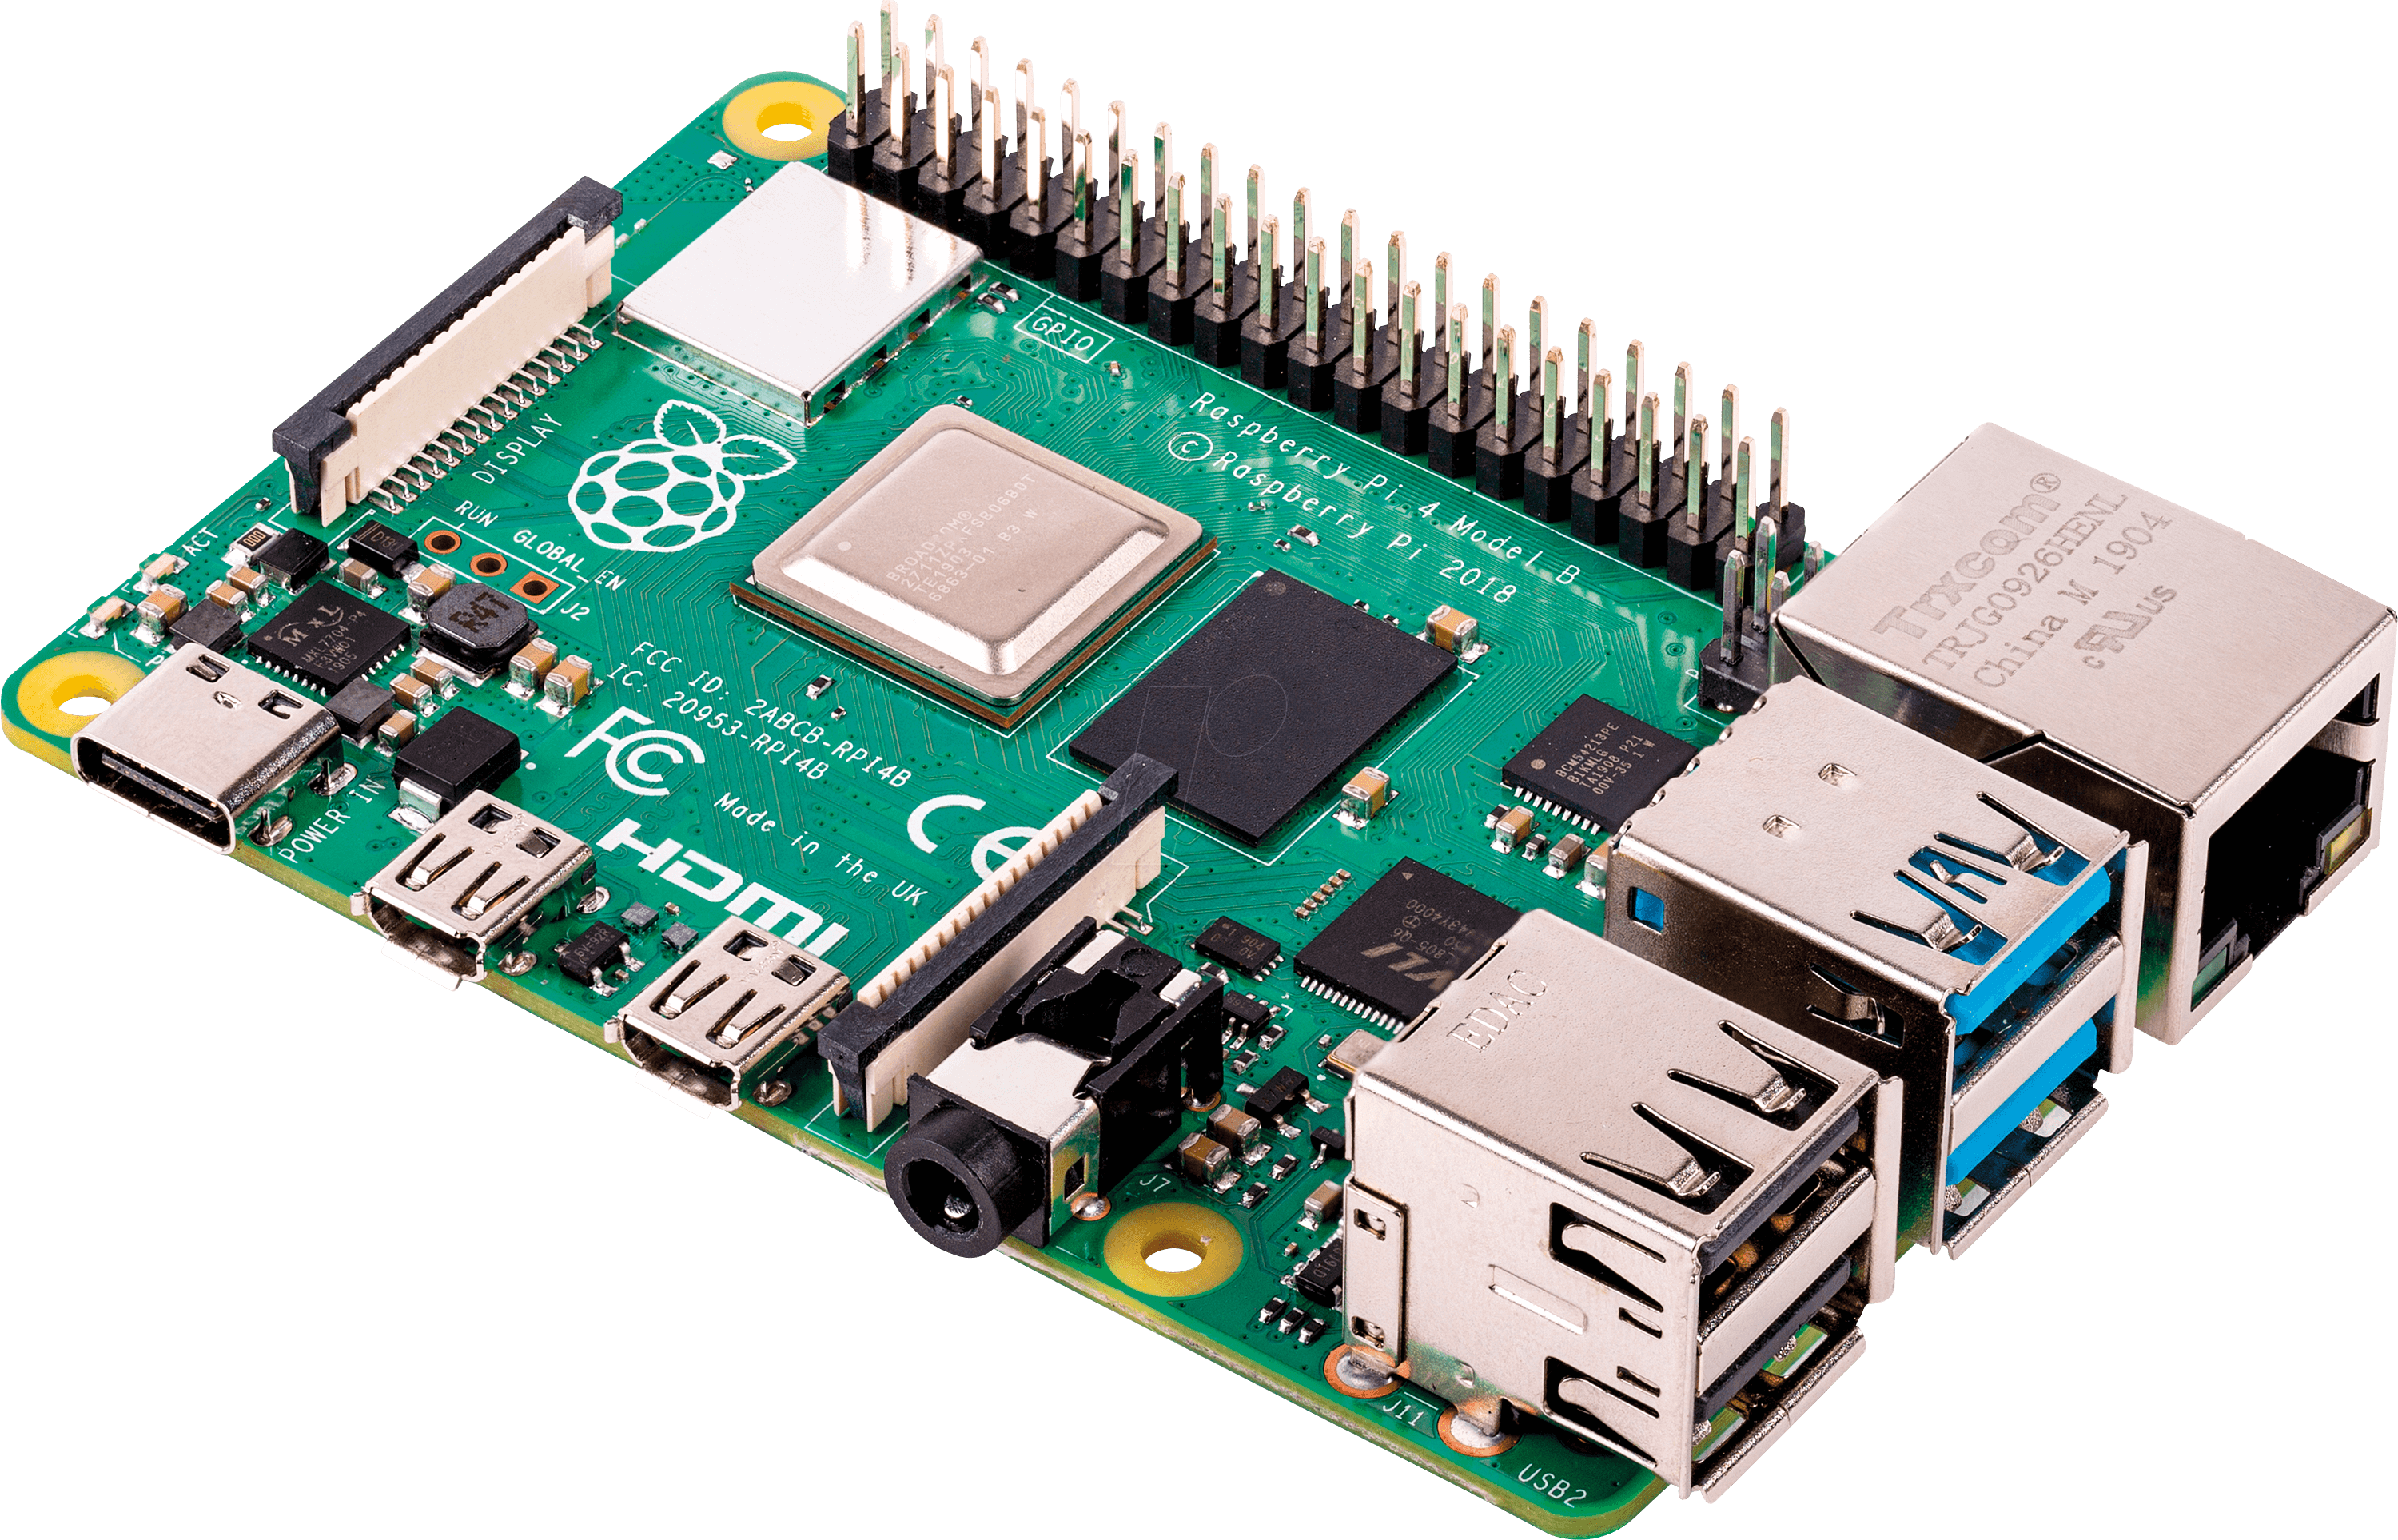
\includegraphics[width=6cm]{./Bilder/raspberrypi_4.png}
    \caption{Raspberry Pi 4}
    \label{img:raspberrypi}
\end{figure}



\subsection*{Kamera}
Verwendet wurde ein Raspberry Pi Kamera Modul mit 5MP OV5647 Sensor 
und automatschem umschalten der Infrarot Funktion der Marke 
Longrunner verwendet.
%https://www.amazon.de/gp/product/B07R4JH2ZV/ref=ppx_yo_dt_b_asin_title_o01_s00?ie=UTF8&psc=1
Dieses verfügt zusätzlich über zwei Infrarot LEDs, mit 850 nm wellenlänge.

\begin{figure}[H]
    \centering
    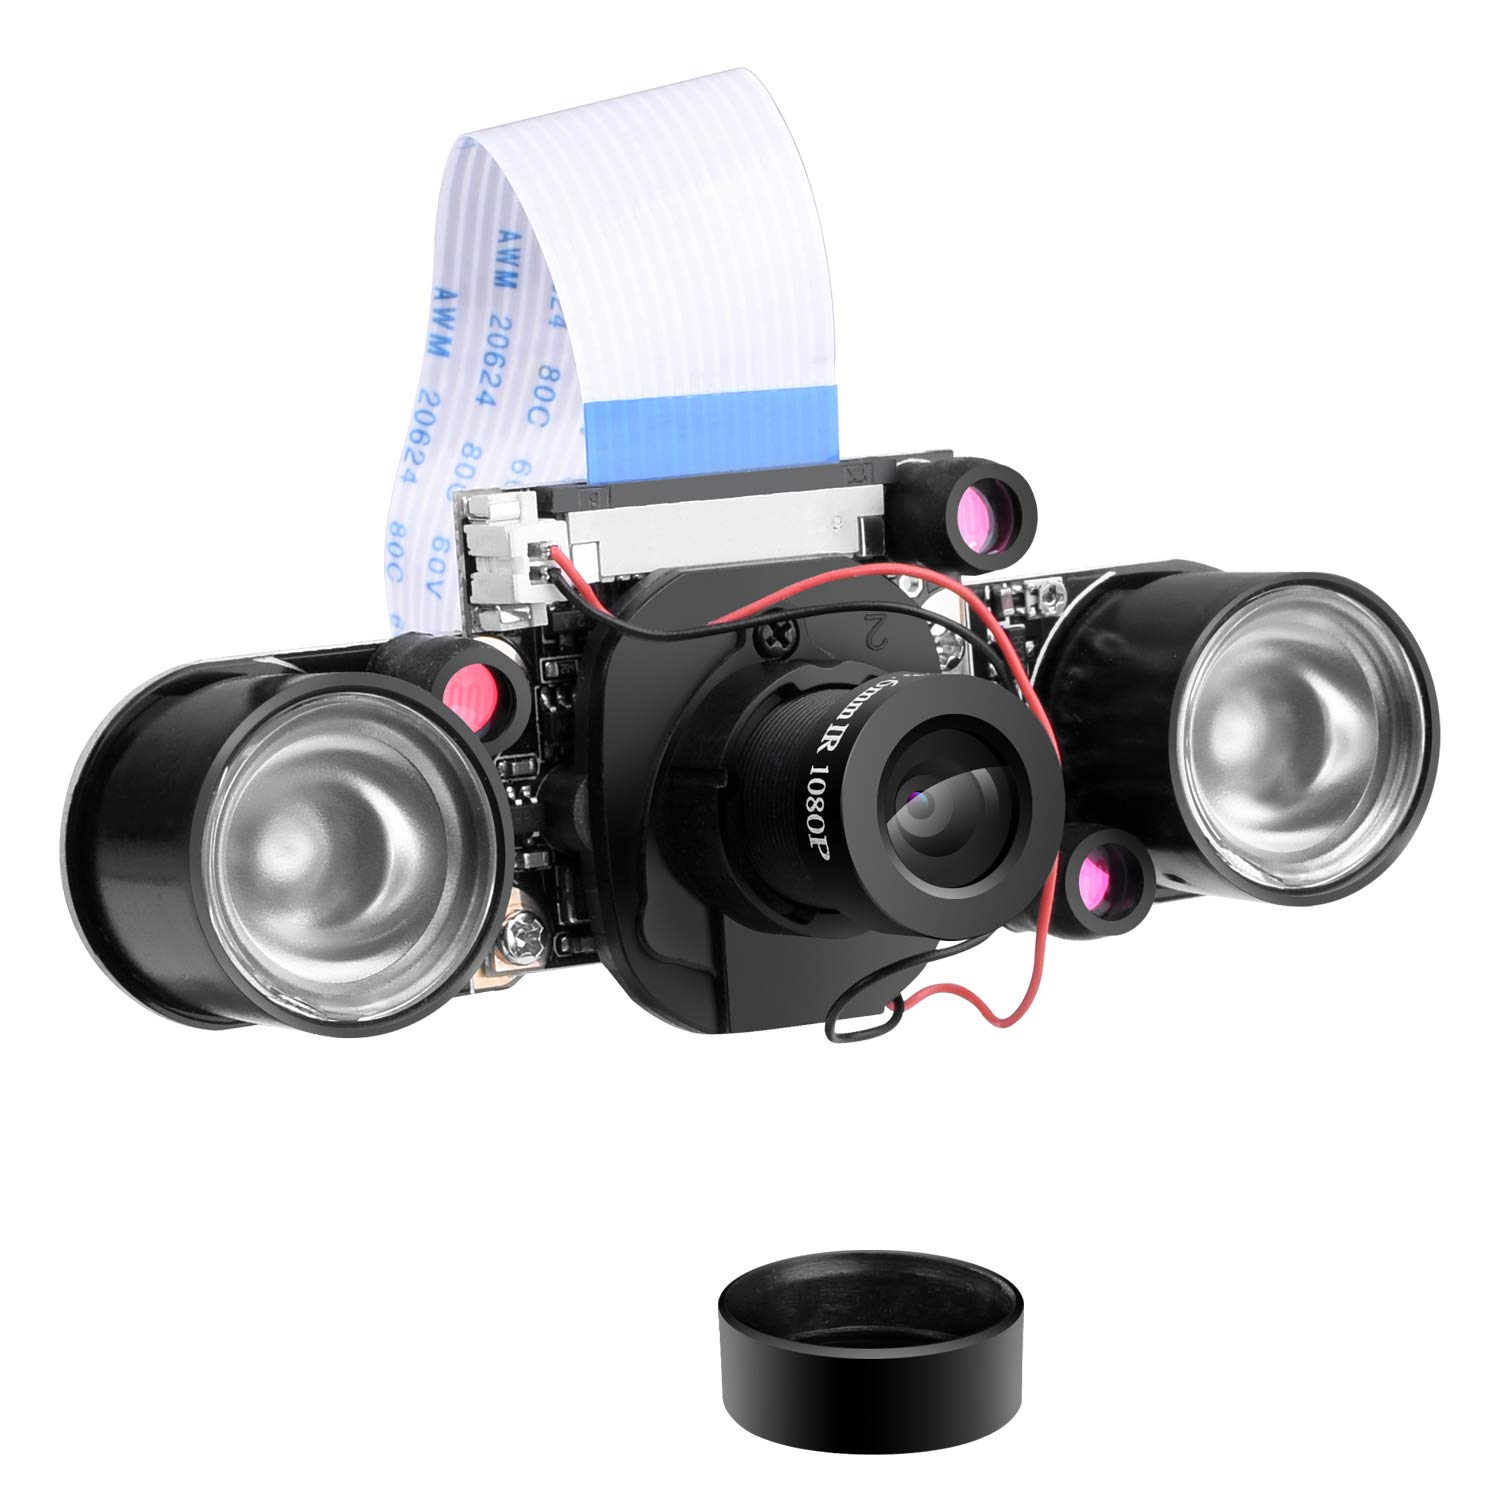
\includegraphics[width=0.35\textwidth]{longrunner.jpg}
    \caption{Longruner for Raspberry Pi 4 Camera Kamera Module}
    \label{fig:rpicam}
\end{figure}

Für das Umschalten in den Infrarot Modus, wird der Infrarot Filder, welcher sich 
für normale Aufnahmen vor der Linse befindet entfern, was über einen magnetschalter 
der mit einem Helligkeitssensor getriggert wird erfolg.

 

\subsection*{sonstiges}
\begin{itemize}
    \item Internet Stick%https://www.amazon.de/gp/product/B00HSZEY34/ref=ppx_yo_dt_b_asin_title_o00_s00?ie=UTF8&psc=1
    \item Hülle
    \item Powerbank
\end{itemize}

\section{Implementierung/Software}

Bestht aus 3 Scripten:

\begin{itemize}
    \item main
    \begin{itemize}
        \item 
    \end{itemize}
    \item detection
    \begin{itemize}
        \item init
        \item motion
        \item create exec net
        \item infer frames
    \end{itemize}
    \item connection
    \begin{itemize}
        \item init
        \item login
        \item connect
        \item send
        \item disconnect
    \end{itemize}
\end{itemize}

\subsection*{Inferenz}


Um nicht durchgehend die Input Frames welche die Kamera liefert inferieren zu 
müssen, wurde mithilfe der Library OpenCV ein bewegungserkennung 
implementiert. Diese speichert bei start der Anwendung ein Frame 
als Refernz ab, und kann damit alle weiteren Input frames vergleiche, 
indem der Abstand der einzelnen Pixel werte berechnet und gemittelt wird.

Der Ablauf der reinen Asynchronen Inferenz ist grob in 
folgendem Pseudocode dargestellt. 


%Asynchrone inferenz
%https://docs.openvinotoolkit.org/latest/_demos_python_demos_object_detection_demo_ssd_async_README.html

% main
% \begin{algorithm}[H]
%     \caption{Main Program}
%     \begin{algorithmic}

%     %\STATE INIT EXEC_NET, CAM

%     \WHILE{\TRUE}
%         \STATE capture frame
        
%         \IF{frame has motion}
%             \STATE $buffer \leftarrow frmae$
%         \ENDIF

%         \IF{buffer is empty}
%             \STATE disconnect
%         \ENDIF

%         \STATE result = inferFrames (buffer)

%         \FOR{all results}
%             \STATE process results
%             \IF {saved}
%                 \STATE sendRequest = \TRUE
%             \ENDIF
        

%             \IF {no detectoin for 20 times}
%                 \STATE reset motion background
%                 \STATE delete buffer
%                 \IF {connected}
%                     \STATE disconnect
%                 \ENDIF
%             \ENDIF

%         \ENDFOR

%         \IF {send all every minute}
%             \STATE save current detections
%             \STATE sendRequest = \TRUE
%         \ENDIF

%         \IF{sendRequest == \TRUE}
%             \IF{not logged in}
%                 \STATE log in
%             \ENDIF

%             \IF{not connected}
%                 \STATE connect
%             \ENDIF

%             \STATE server, port $\leftarrow$ connection

%             \STATE sendRequest = \FALSE
%             \FOR{all saved images}
%                 \IF{send image $\rightarrow$ server, port}
%                     \STATE delete image
%                 \ELSE
%                     \STATE sendRequest = \TRUE
%                 \ENDIF
%             \ENDFOR

%         \ENDIF
%     \ENDWHILE


%     \end{algorithmic}
% \end{algorithm}


% inferenz
\begin{algorithm}[H]
    \caption{Asynchrone Inferenz}
    \begin{algorithmic}
    \WHILE{\TRUE}
        \STATE capture Frame
        \IF{Frame has Motion}
            \STATE Buffer $\leftarrow$ Frame
        \ENDIF
        \FOR{$reqId$ = 0 to $reqMax$}
            \IF {Model.reqests[$reqId$].wait(0)}
                \STATE result = Model.reqests[$reqId$].output
                \STATE inferedFrames $\leftarrow$ (result, currentFrames[$reqId$])
                \IF {Buffer not empty}
                    \STATE currentFrames[$reqId$] $\leftarrow$ Buffer 
                    \STATE inFrame = preprocess: currentFrames[$reqId$]
                    \STATE Model.inferAsync($reqId$, inFrame)
                \ENDIF
            \ENDIF
        \ENDFOR
        \RETURN inferedFrames
    \ENDWHILE
    \end{algorithmic}
\end{algorithm}

wobei die wait Funktion mit Timeout = 0 nicht blockierend ist.

Dadurch war es möglich trotz langsamerer inferenz zeit als 
capture zeit, durch zwischenspeichern alle frames zu inferieren, 
unter der Annahme, das nur zeitweise bewegung erkannt und damit 
inferiert werden muss.



\subsection*{Connection}

\begin{itemize}
    \item remote Proxy verbinung über SSH
    \item mit SCP Protokol send
\end{itemize}





